\documentclass[t]{beamer}
% \documentclass[handout,xcolor=pdftex,dvipsnames,table]{beamer}

\mode<presentation>
{
  \usetheme{Warsaw}
  \usecolortheme{whale}
  % or ...

  % or whatever (possibly just delete it)
  \setbeamertemplate{navigation symbols}{}
}

\usepackage{hyperref}


% make a command to decrease font size locally when desired
\newcommand\Fontvi{\fontsize{8.5}{7.2}\selectfont}



\setbeamertemplate{itemize items}[ball]
\setbeamertemplate{itemize subitem}[triangle]
\setbeamertemplate{itemize subsubitem}[circle]
\setbeamercovered{invisible}

\usepackage{palatino} 
\usepackage{listings} % Gives syntax highlighting for python code. 
\usepackage{color} % Used for syntax highlighting. 
\usepackage{textcomp} % Used for syntax highlighting. 
\usepackage{caption}
\captionsetup{labelformat=empty,labelsep=none}
% This gives syntax highlighting in the python environment 
\definecolor{gray}{gray}{0.5} 
\definecolor{key}{rgb}{0,0.5,0} 
\lstset{
language=python,
basicstyle=\ttfamily\tiny, 
otherkeywords={1, 2, 3, 4, 5, 6, 7, 8 ,9 , 0, -, =, +, [, ], (, ), \{, \}, :, *, !}, 
keywordstyle=\color{blue}, 
stringstyle=\color{red},
showstringspaces=false,
alsoletter={1234567890},
otherkeywords={\ , \}, \{},
keywordstyle=\color{blue},
emph={access,and,break,class,continue,def,del,elif ,else,%
except,exec,finally,for,from,global,if,import,in,is,%
lambda,not,or,pass,print,raise,return,try,while},
emphstyle=\color{black}\bfseries,
emph={[2]True, False, None, self},
emphstyle=[2]\color{green},
emph={[3]from, import, as},
emphstyle=[3]\color{blue},
upquote=true,
morecomment=[s]{"""}{"""},
commentstyle=\color{gray}\slshape,
emph={[4]1, 2, 3, 4, 5, 6, 7, 8, 9, 0},
emphstyle=[4]\color{blue},
literate=*{:}{{\textcolor{blue}:}}{1}%
{=}{{\textcolor{blue}=}}{1}%
{-}{{\textcolor{blue}-}}{1}%
{+}{{\textcolor{blue}+}}{1}%
{*}{{\textcolor{blue}*}}{1}%
{!}{{\textcolor{blue}!}}{1}%
{(}{{\textcolor{blue}(}}{1}%
{)}{{\textcolor{blue})}}{1}%
{[}{{\textcolor{blue}[}}{1}%
{]}{{\textcolor{blue}]}}{1}%
{<}{{\textcolor{blue}<}}{1}%
{>}{{\textcolor{blue}>}}{1},%
numbers=none,
}

\newcommand{\putat}[3]{\begin{picture}(0,0)(0,0)\put(#1,#2){#3}\end{picture}}



\title[]{Python Workshop\\
 \includegraphics[scale=0.055]{figures/python-app.png}\hspace{5 pt}How we use python\hspace{5 pt}\includegraphics[scale=0.055]{figures/python-app.png} }

\author[Fienen] % (optional, use only with lots of authors)
{Mike~Fienen}
\institute[USGS] % (optional, but mostly needed)
{
  U.S. Geological Survey\\
  Wisconsin Water Science Center, Middleton, Wisconsin USA
  }
  \titlegraphic{\includegraphics[scale=0.5]{figures/c_USGSid1.pdf}}
  

\date[UQ12] % (optional, should be abbreviation of conference name)
{USGS National Groundwater Workshop, August 2012}

\subject{Python}


\begin{document}

\begin{frame}
  \titlepage
\end{frame}
\logo{\vspace{-0.3cm} \includegraphics[width=1.5cm]{figures/c_USGSid1.pdf}\hspace*{11.10cm}}  

\begin{frame}{How we use python}
\tableofcontents
\end{frame}

\section{Social.Water}
\begin{frame}[fragile]
\frametitle{Social.Water}
Social.Water is a citizen-science project in support of CrowdHydrology. The code is all written in Python.
\begin{center}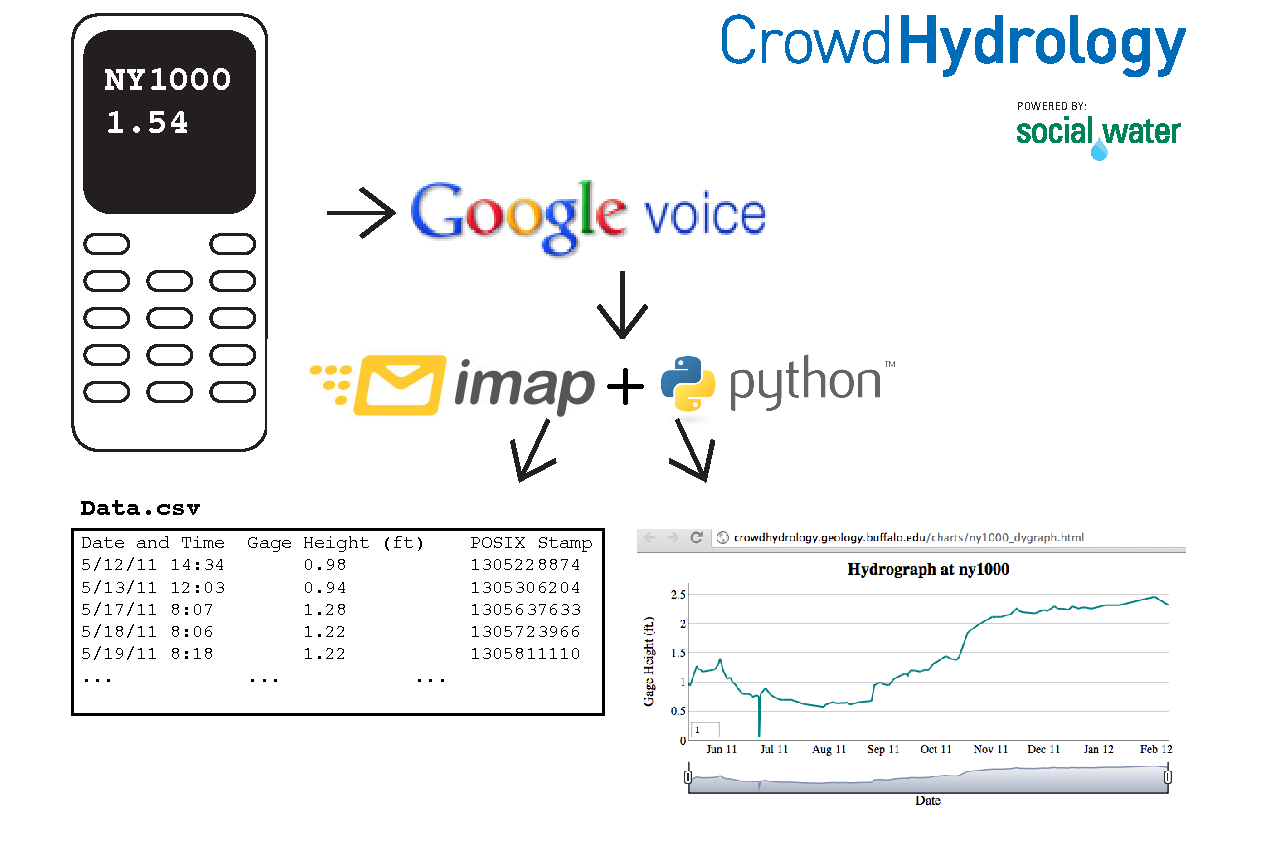
\includegraphics[scale=.4]{figures/socialwater1.pdf}\end{center}
\end{frame}

\begin{frame}[fragile]
\frametitle{Social.Water---What Python Provides}
\begin{columns}[l]
\column{.6\textwidth}

\begin{itemize}
\item Decrypt a password
\item Log in to IMAP email account
\item Read all new messages
\item Parse all new messages
\item Perform fuzzy search on gage \#
\item Write and display results on Web

\end{itemize}

\column{.4\textwidth}
\begin{center}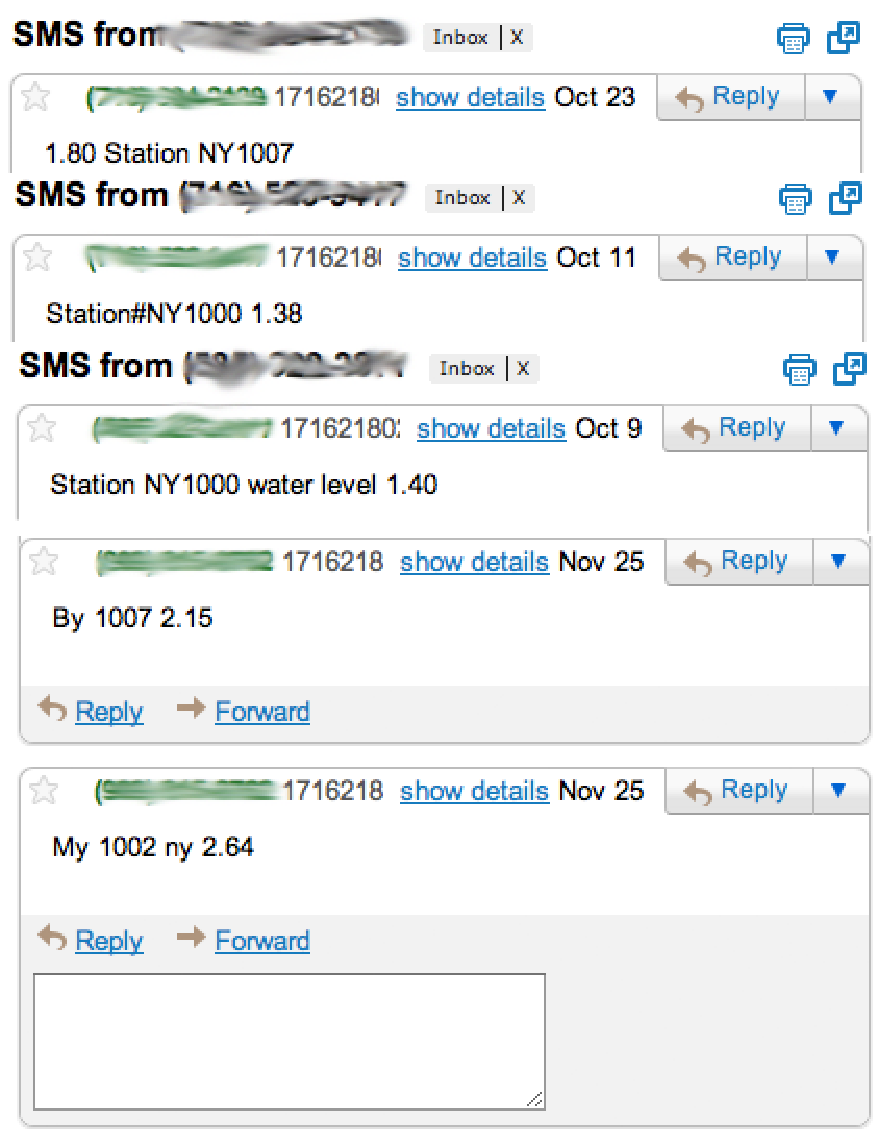
\includegraphics[scale=.3]{figures/SW_msg.pdf}\end{center}

\end{columns}
\end{frame}

\section{cloudPEST}
\begin{frame}[fragile]
\frametitle{cloudPEST}
\begin{center}\includegraphics[scale=.3]{figures/COVERcloudPEST.pdf}\end{center}

\end{frame}
\end{document}